\chapter{Sekwencjonowanie i adnotacja genomu}
\label{section:biologiny_wstep}

\section{Sekwencjonowanie i asembling DNA}
Sekwencjonowanie to jedna z technik biologii molekularnej, pozwalająca na odczytanie kolejności nukleotydów w cząsteczce DNA.

Najlepiej byłoby, gdyby projekt genomu reprezentował kompletną sekwencję nukleotydową wszystkich chromosomów danego gatunku. 
Jednak w rzeczywistości, istnieje wiele potencjalnych problemów związanych z procesem sekwencjonowania. Nie istnieje bowiem, jedna, prawdziwa sekwencja dla gatunku z powodu indywidualnej zmienności genetycznej jednostek. 
Nawet komórki tego samego osobnika mogą różnić się w zawartości genetycznej z powodu mutacji somatycznych. Złożony genom będzie tylko jedną reprezentacją wariacji występującej u danego gatunku. 
Zasadniczo sekwencjonuje się tylko jednego osobnika, ale czasami genom stanowi konsensus wielu połączonych próbek (projekt HUGO). 
Należy zdawać sobie sprawę, że procesowi sekwencjonowania zawsze będą towarzyszyć błędy na poziomie poszczególnych nukleotydów oraz ich kolejności (błędy montażu). 
Każdy złożony genom jest wynikiem serii złożeń metodami heurystycznymi i powinien być traktowany jako robocza hipoteza.

\begin{figure}[h]
	\centering
	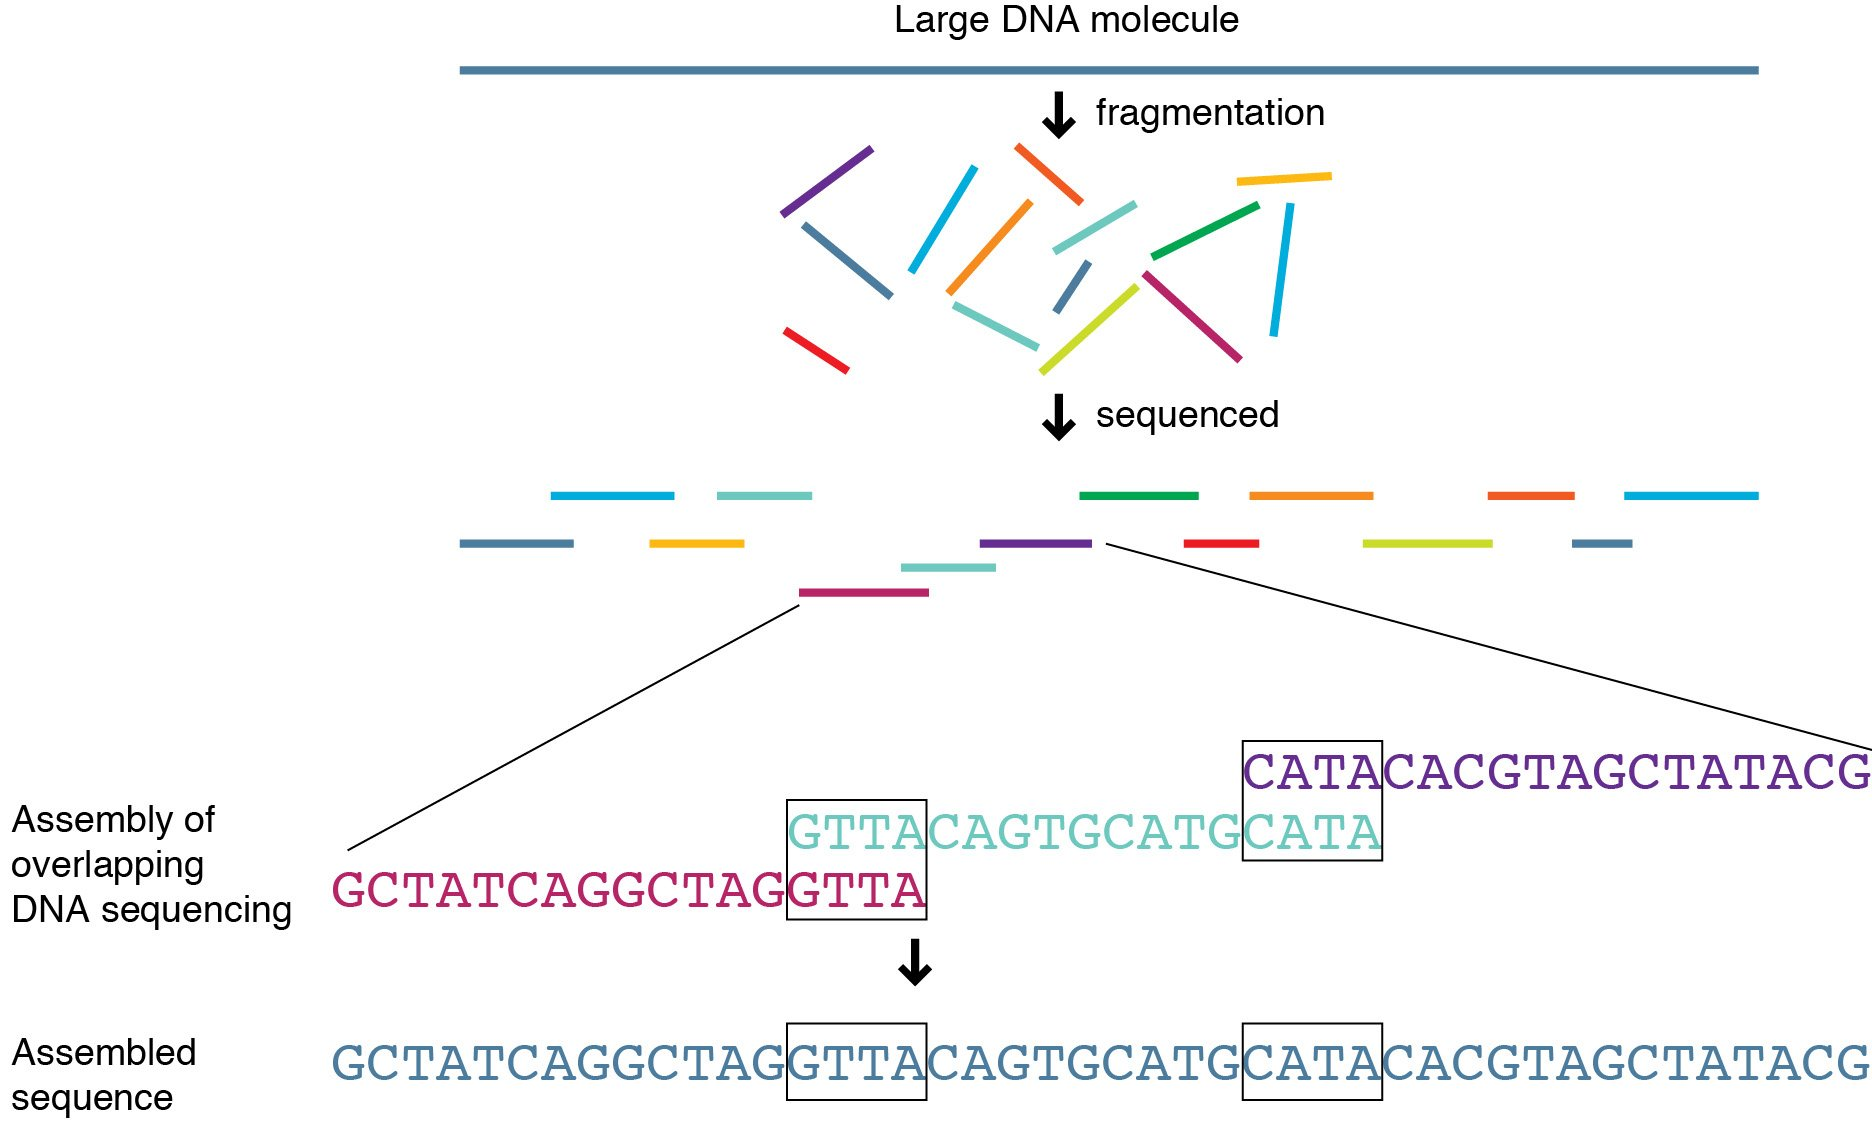
\includegraphics[width=0.9\textwidth]{img/sequenctioning-process.png}
	%zdjecie z %http://knowgenetics.org/whole-genome-sequencing/
	\caption{Schemat sekwencjonowania}
	\vspace{-0.5cm}
	\caption*{\scriptsize Źródło: \url{http://knowgenetics.org/whole-genome-sequencing/}}
	\label{img:schemat-sekwencjonowania}
\end{figure}

Większość projektów, w początkowej fazie sekwencjonowania kieruje się strategią polegającą na losowym pocięciu DNA na bardzo małe fragmenty.
W zależności od wykorzystanej technologii, fragmenty mogą mieć różne długości. Istnieje trend w kierunku przeprowadzania odczytów technikami dającymi coraz krótsze fragmenty. 
Tradycyjne sposoby (Sanger) dawały fragmenty długości około 1000 par zasad. Obecnie wykorzystywane techniki dające najkrótsze rezultaty osiągają wyniki rzędu dziesiątek pz. (SOLiD, Illumina - rys.\ref{img:sekwencjoner-illumina}).

\begin{figure}[h]
	\centering
	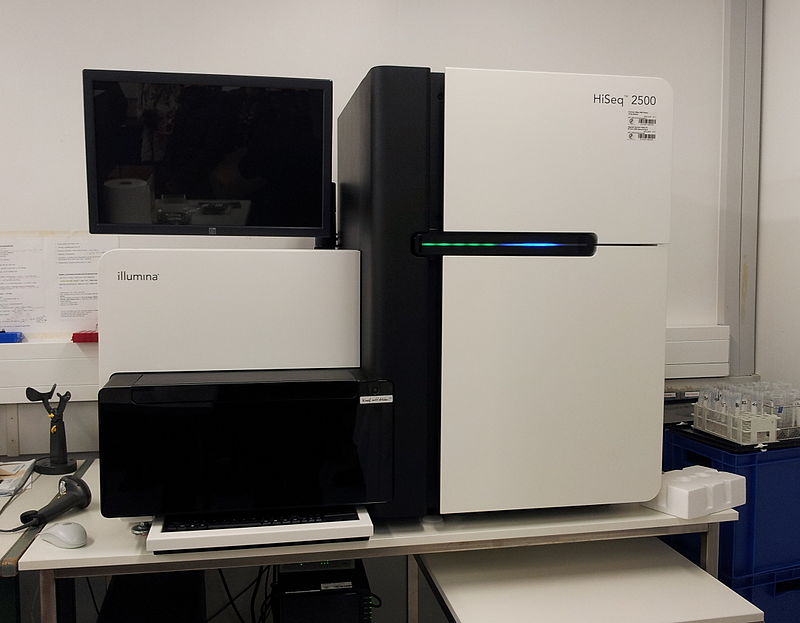
\includegraphics[width=0.75\textwidth]{img/sekwencjoner-illumina.jpg}
	%zdjecie z http://wiedza.alkahest.umcs.pl/jak-limfocyty-t-przekazuja-informacje/
	\caption{Sekwencjoner Illumina HiSeq 2500}
	\vspace{-0.5cm}
	\caption*{\scriptsize Źródło: \url{http://wiedza.alkahest.umcs.pl/jak-limfocyty-t-przekazuja-informacje/}}
	\label{img:sekwencjoner-illumina}
\end{figure}

Następie, w procesie asemblingu, fragmenty sekwencji są składane w dłuższe odcinki. Dobór algorytmu jest zależny od długości odcinków zsekwencjonowanych w poprzednim etapie. Jest to proces skomplikowany i wykorzystywane są do tego zasobożerne programy. 
Efektem początkowego składania sekwencji są kontigi.
Na dalszych etapach, po analizach wykorzystujących biblioteki dłużych sekwencji DNA, kontigi są zespalane w struktury zwane skafoldami.
Mają one zazwyczaj postać sekwencji z lukami o znanej długości - dziury oznaczane są znakiem ,,N''.

\section{Adnotacje}

\section{Prezentacja danych}

\section{Przegląd literatury}